\section{Methodology}
\subsection{Overview}
This project consists of three main units: a discharge flow control unit, a discharge collection  unit, and a main control unit. 
\subsection{Discharge flow control unit}
\par
The unit is used for controlling the flow rate at the end of the pipe system ideally by allowing a regulated amount of water into the collection tank. To ensure little modification to the current state-of-the-art machine, the flow control unit utilizes the existing ball valve to achieve this operation. Furthermore, to attain the regulated flow, the valve aperture opens and closes in small and precise steps as specified by the user. Therefore, to achieve this, the servo motor, hosted on a motor cage and clamped to the valve, is coupled to the ball valve with help of an interface and controlled by a driver based on the STM32F40VET6 microcontroller.  
\subsection{Design Consideration}
Precision in the opening and closing of the ball valve is key to ensuring that only the required amount of water is collected within the stipulated time. Servo and stepper motors were considered to achieve this operation.
\subsubsection{Stepper Motor}
\par
The motor operates by accurately synchronizing position with the pulse signal output from the controller to the driver, achieving highly accurate positioning and speed control. Stepper motors feature high torque and low vibration at low speeds ideally below 1500rpm, ideal for applications requiring quick positioning in a short distance. Furthermore, stepper motor rotates with a fixed step angle typically 1.8 degrees for a 2-phase. However, to achieve this requires the use of a micro-step driver.
\par
Besides, while having full control of rotation and speed, the simple structure of stepper motors is achieved without using electrical components, such as an encoder within the motor. For this reason, stepper motors are very robust and have high reliability with very few failures. As for stopping accuracy, ±0.05° (without cumulative pitch errors) is very accurate. Because the positioning of stepper motors is performed by open-loop control and operated by the magnetized stator and magnetic rotor with small teeth, stepper motors have a higher follow-up mechanism toward commands than that servo motors. Also, no hunting occurs when stopping stepper motors. 
\subsubsection{Servo Motor}
\par
Servo motors run significantly faster than stepper motors, with speeds greater than 1500rpm. This enables servo motors to be used with gearboxes to deliver much higher torque at useful speeds. They also deliver more consistent torque across the speed range of the motor. Unlike stepper motors, they do not have holding torque per se. Closed-loop operation enables the controller/drive to command that the load remain at a specific position, however, and the motor will make continual adjustments to hold it there. Thus, servo motors can deliver de facto holding torque. The Servo motor rotates with a fixed step angle as low as 1 degree with or without the use of a driver. Furthermore, when powered, servo motors tend to move their shaft position to the zero position, a phenomenon referred to as hunting.
\subsection{Justification}
\par
Servo motor is used in the discharge flow control unit because of the small step angle (1 degree) that it can turn as compared to a stepper with a typical step angle of 1.8 degrees. The smaller the angle, the more the number of steps hence the experiment could be conducted as many times as possible for higher accuracy. Furthermore, the fact that servo motors do not necessarily need a micro-step driver for their operation reduces the overall cost.
\subsection{Flow Control Unit Designs}
\begin{figure}[ht]
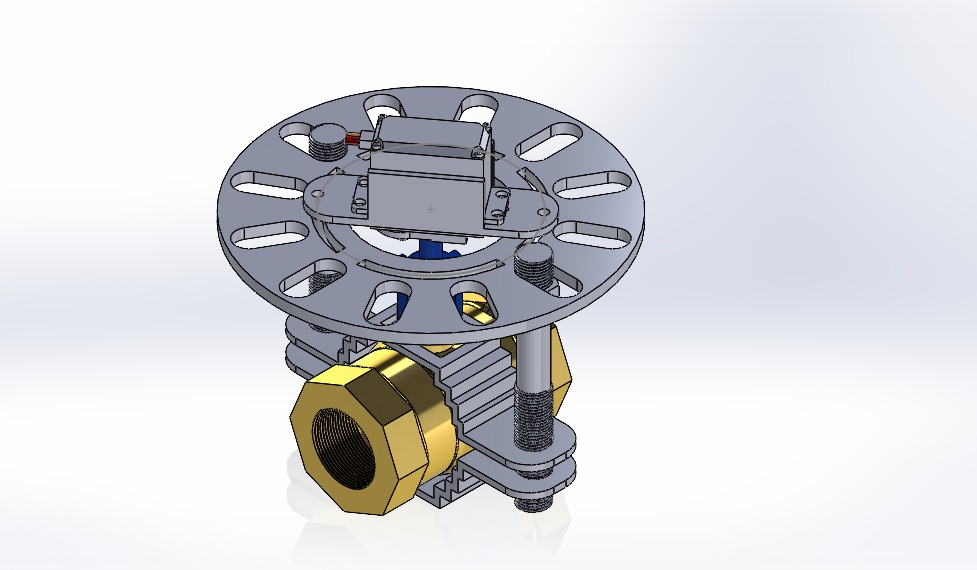
\includegraphics[width=0.9\linewidth]{Figures/Image3.jpeg}
\centering
\caption{Top View }
\label{fig:Image3}
\end{figure}

\begin{figure}[ht]
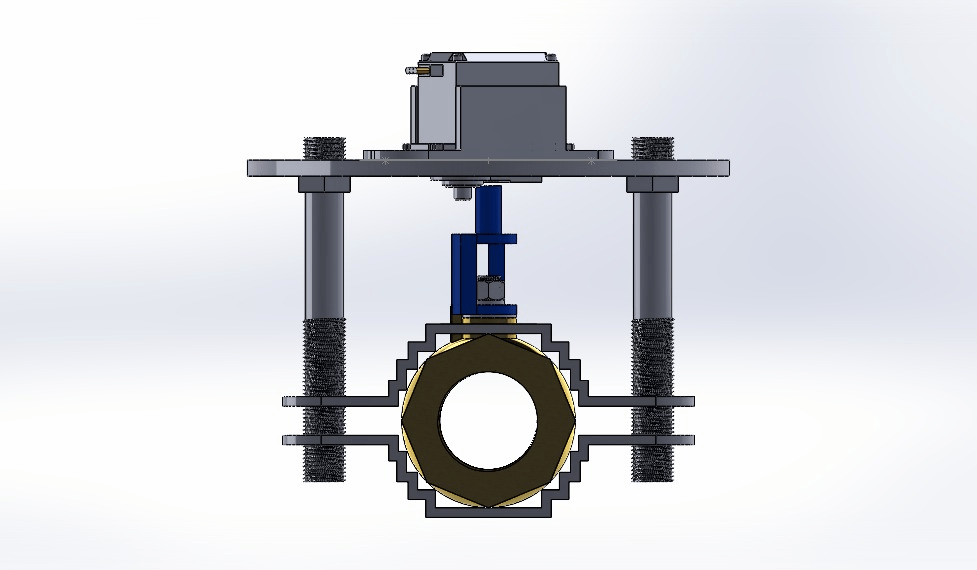
\includegraphics[width=0.9\linewidth]{Figures/Image1.png}
\centering
\caption{Top View }
\label{fig:Image1}
\end{figure}

\subsection{Discharge collection unit}
It is the core part of the experiment. The discharge collection unit comprises the flow diversion sub-unit, a discharge collection tank, an outlet valve, and weight and temperature measurements sub-units.
\subsubsection{Flow diversion sub-unit}
\par
The sub-unit is responsible for diverting the discharge from the main pipe system to either the collection tank or into the main reservoir. The weight of the collected discharge is critical to the whole process. Therefore, to ensure that only the required amount of water is collected, the diversion unit ensures that there are minimal splashes and leakages by use of a curved flap. Furthermore, the fast response of the unit is attained by the use of an electromagnet whose linear motion is amplified by the use of a lever system hence providing the flap with a wider angle.
\subsection{Design Consideration}
The sub-unit is to have a faster response and large linear displacement capabilities Piezoelectric actuators and electromagnets were considered for this application.
\subsubsection{Piezoelectric Actuators}
\par
Piezoelectric actuators are transducers that convert electrical energy into a mechanical displacement or stress based on a piezoelectric effect, or vice versa. They are used widely as a high precision positioning mechanism since they can control a small mechanical displacement at high speed, with the advantages of large generated force, stable displacement, and ease of use. However, problems include insufficient displacement and the large voltage up to a few hundred volts, which is needed.
\subsubsection{Electromagnets}
\par
Electromagnetic devices leverage the unique ability of magnetic metals such as iron to generate a magnetic field when electric current is applied. One of the biggest advantages offered by electromagnetic devices is durability. Unlike piezoelectric devices, which have the potential for shattered crystals, or electrostatic solutions with their required precise measurements, electromagnetic offerings can withstand high-volume, high-intensity use without suffering output or capacity loss. This makes them ideal for applications in which on-demand power and magnetism are required. Furthermore, as compared to piezoelectric actuators, electromagnets have a faster response and larger displacements which is actually ideal for our application.
\subsection{Justification}
\par
Electromagnets is used as the main actuation mechanism for the flow diversion sub unit due to its faster response when energized as compared to piezoelectric actuators. Furthermore, piezoelectric actuators produce very small mechanical linear displacements as compared to electromagnets.
\subsection{Flow Diversion Sub-Unit Designs}

\begin{figure}[ht]
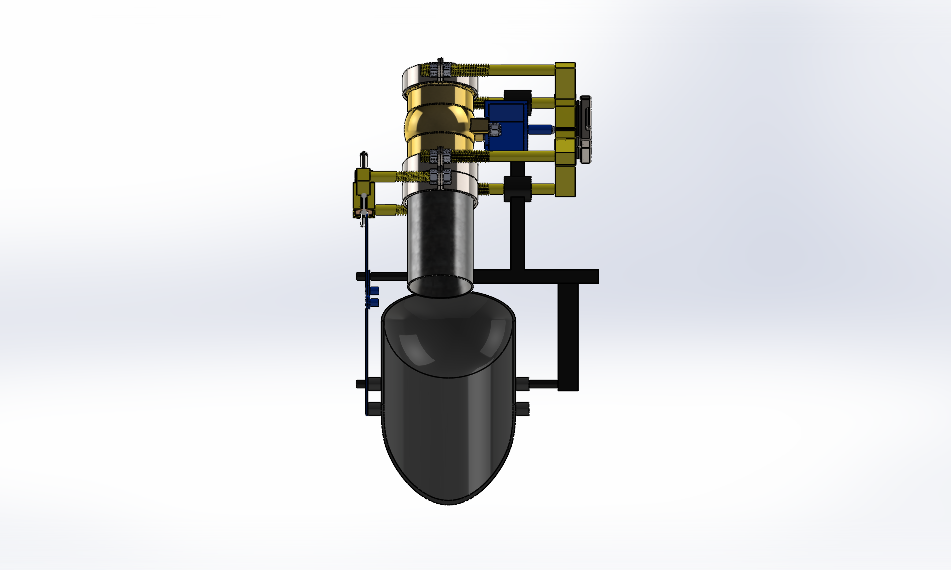
\includegraphics[width=0.9\linewidth]{Figures/DiversionUnit_front.png}
\centering
\caption{Diversion Unit front View }
\label{fig:DiversionUnit_front.}
\end{figure}


\begin{figure}[ht]
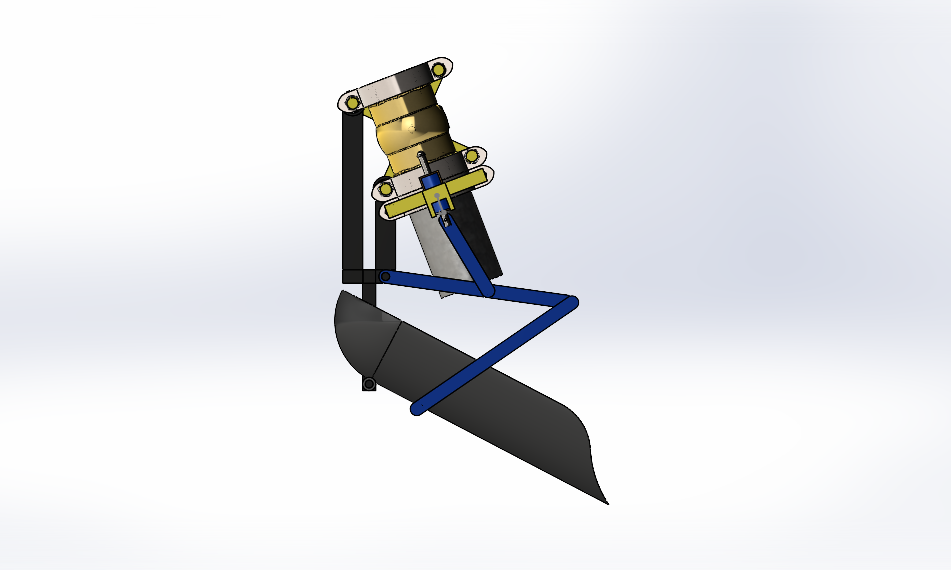
\includegraphics[width=0.9\linewidth]{Figures/DiversionUnit_side.png}
\centering
\caption{Diversion Unit side View }
\label{fig:Diversion Unit_side}
\end{figure}

\begin{figure}[ht]
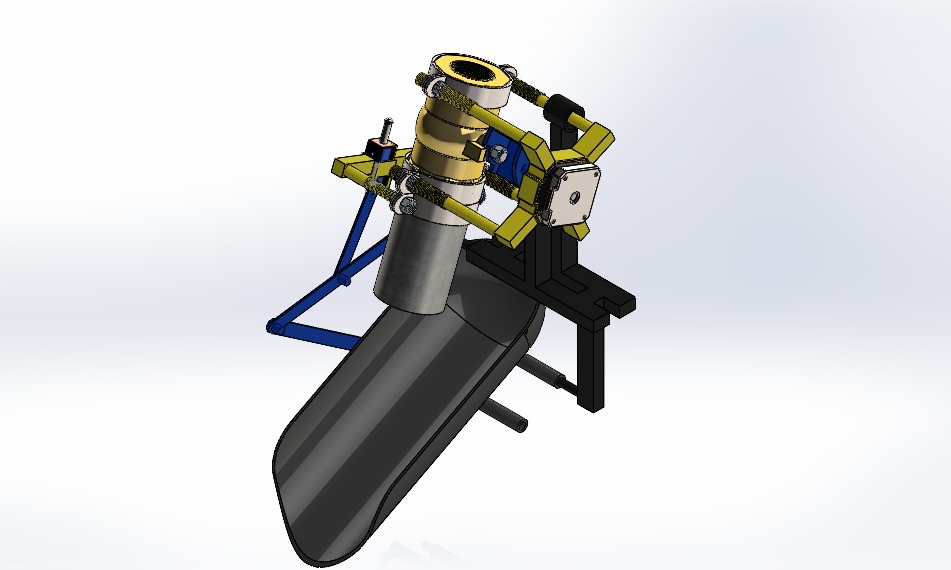
\includegraphics[width=0.9\linewidth]{Figures/DiversionUnit_isometric.png}
\centering
\caption{Diversion Unit isometric View }
\label{fig:Diversion Unit isometric}
\end{figure}




\subsubsection{Discharge collection tank}
This unit will be used to collect the discharge temporarily at each step during the experiment. The weight and temperature of the discharge will be measured within the tank. The design of the tank will involve the consideration of the following factors :
\begin{enumerate}
    \item Position \newline
    The position of the tank will influence size of the collection pipe and also the positioning of the outlet valve. The tank will be required the elevated above the reservoir in order to eliminate the need for a pump for pump out the discharge. 
    \item Insulation \newline
    Since the temperature of the discharge is taken in this tank, the influence of the external environment will have a negative impact on the readings. The tank is therefore required to maintain internal environment with minimal effect from the external environment. 
    \item Shape \newline 
     The shape of the tank will determine will influence weight measurement, and the positioning of the outlet valve.
\end{enumerate}
\subsubsection{Outlet valve}
This valve will be responsible to emptying the discharge collection tank into the reservoir. The design of this valve will be based on the following factors :
\begin{enumerate}
    \item Position \newline 
    The position of the outlet valve will be critical since it determines how fast the mini collection tank drains into the reservoir.
    \item Size. \newline
    The size of the valve will also determine how fast the tank empty to the reservoir. 
\end{enumerate}
\subsubsection{Weight measurement sub-unit}
This sub-unit will be used to measure the weight of the discharge in the collection tank. The following approaches will be considered for this unit :

\begin{enumerate}
    \item Ultrasonic \newline
    Ultrasonic waves will be used to determine the depth of the discharge in the tank. This will be used with the cross-sectional area of the tank, and the density of the tank to determine the weight of the discharge based on following equation.
    \item Load cells \newline
    This will utilize load cells distributed below the discharge collection tank. The average of the output of the load cells will be averaged. 
\end{enumerate}

\par
The choice between these two approaches will depend on the following factors :
\begin{enumerate}
    \item Resolution. \newline
    The refers to the smallest unit that can be measured by the measurement device. The resolution of ultrasonic waves will depend on the pulse rate of the ultrasonic wave generator. 
    \item Reliability. \newline
    The application of ultrasonic waves requires the consideration of other factors such as the cross-sectional area and the shape of the tank. This will not be the case with the load cells. This makes the measurements using the load cells more reliable than those utilizing ultrasonic waves.
\end{enumerate}

\subsubsection{Temperature measurement sub-unit}
This sub-unit will be required to measure the temperature of discharge in the tank. The following types of temperature measurement methods will be considered in the choice of a suitable sub-unit:
\begin{enumerate}
    \item Contact temperature measurement \newline
    The measuring device will be placed inside the tank and thus it will come into contact into contact with the discharge.
    \item Contactless temperature measurement \newline
    In the non contact type, the measuring device  will not come into contact with the discharge.
\end{enumerate}
\par
The choice between the two technologies will be based on the following :
\begin{enumerate}
    \item Sensitivity \newline 
     This refers to how responsive the device is to the smallest change in the environment. A contact temperature measurement unit is predicted to have a higher sensitivity as compared to a contactless unit.
     \item Reliability \newline
     The application of a contactless temperature unit will require the consideration of the stimuli between the unit and the environment being probed. This is not the case with a contact temperature measurement unit as there is a direct interface with the environment being probed.
\end{enumerate}

\subsection{Interface and Control}
 This unit will take user input through an interface, and process the input with the data from the system using an application logic running in a micro-controller. The application logic will be as shown in figure \ref{fig:control_flow}. The results of the process will be displayed on the interface. 
\begin{figure}
    \centering
    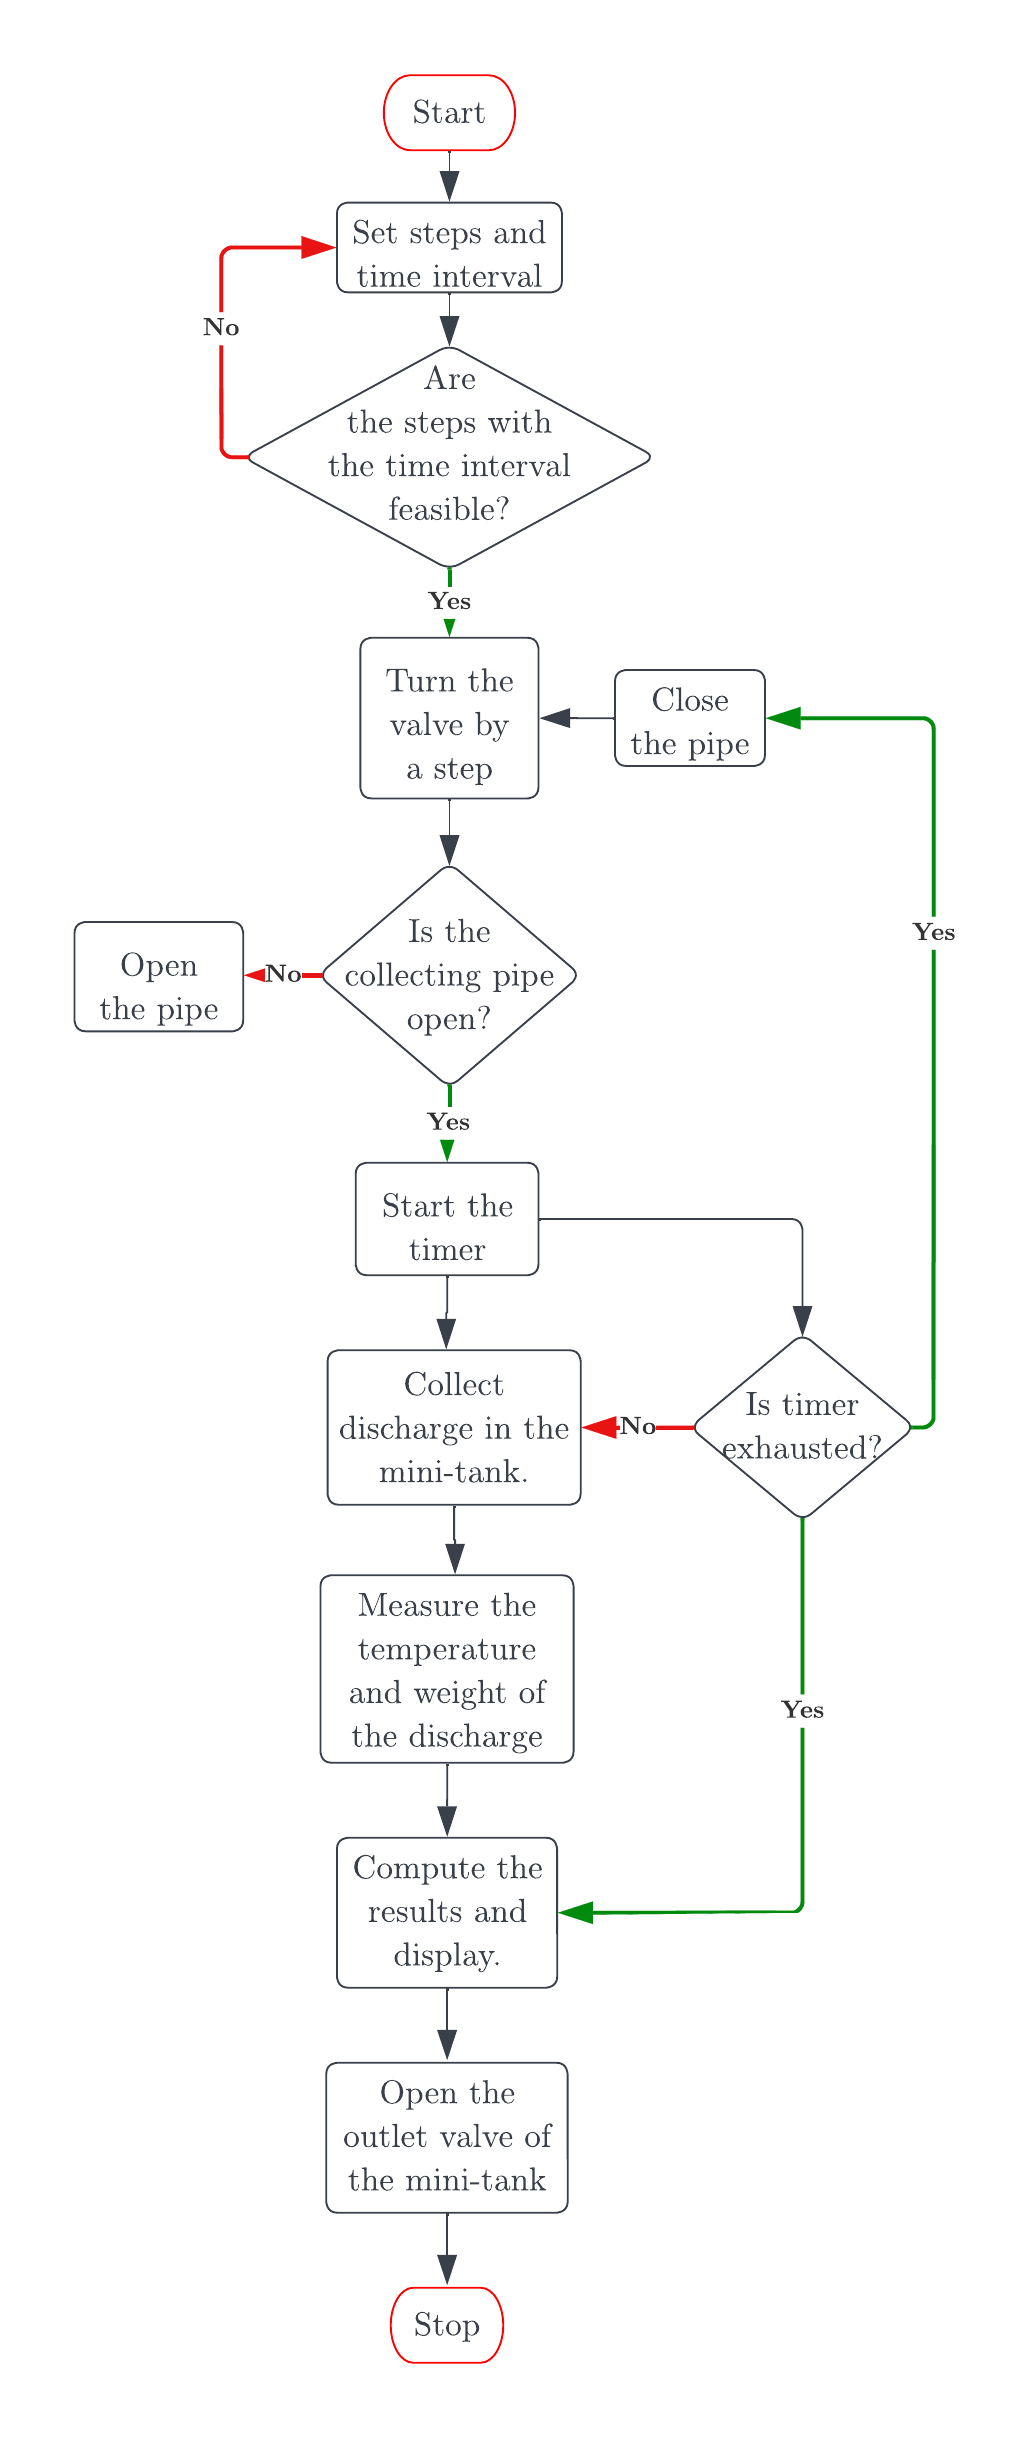
\includegraphics[width=\textwidth,height=\textheight,keepaspectratio]{Figures/Control_flow.png}
    \caption{Application logic}
    \label{fig:control_flow}
\end{figure}
\subsubsection{Processing sub-unit}
This sub-unit executes the application logic, send instructions to the actuators, and reads inputs from sensors in the system. A micro-controller or a fully developed computer board such as Raspberry Pi may be considered for this application. The choice of a micro-controller or a computer chip will be determined by the following factors. 
\begin{enumerate}
    \item \ac{GPIO}s \newline
    These form the primary interface between a micro-controller and the external circuitry. They can be used for several purposes such as analog signal I/O, counter/timer, digital signal I/O, and serial communication. A group of these pins forms a port. The number of pins and hence the size of the port are two important factors that are to be considered in the choice of a micro-controller. 
    \par
    Some devices such as LCD displays with touch capability require bigger ports as many devices require many GPIOs to control them. 
    \item Processing Power  \newline
    This refers to the processing capacity of a micro-controller. A multi-core processor is faster and consumes more power as compared to a single-core processor. A multi-core processor can also render intense graphics on displays. The amount of input processing will guide one in choosing the best micro-controller or microprocessor for the task.
\end{enumerate}
\subsubsection{Interface}
This will provide for a human machine interaction. It will allow one to enter the required experiment parameters like start and stop or reset of the experiment, and read the processed results which will include parameters such as the weight and temperature of the discharge. Some of the interfaces that will be considered in this project are:
\begin{enumerate}
    \item \textbf{LCD with Keypad} \newline
    One can navigate, read and provide input where it is required on the LCD display using the keypad. 
    \item \textbf{LCD with touch capability} \newline
    One can navigate the interface easily by touching and using a virtual keyboard to provide input.
    \item \textbf{LCD with Knobs} \newline
    The interface will be entirely controlled by knobs, navigation from page to page, and parameter input.
\end{enumerate}

The choice of one of the three means to interface with the machine will entirely depend on the following factors.

\begin{enumerate}
    \item Aesthetics \newline
    This refers to the perception of the user while operating the interface. A touch screen is minimalistic, and its aesthetics can be improved easily by adding relatively beautiful graphics in the software. This might not be the case with the case of LCD with knobs. Any attempts to improve its aesthetics might require the addition of knobs. This might clutter the interface.
    \item Ergonomics \newline
    This refers to the impact of the interface on the user, and the ease of operation. LCD display with a keypad interface can be operated even in a moist environment. This might not be the case with an LCD display with touch capability.    
    \item Size  \newline
    This refers to the size of the display with regard to the size of the contents to be displayed. Fewer contents can fit any of the mentioned displays but the operability of the contents in the display should be considered. 
\end{enumerate}